\documentclass[a4paper]{article}
\usepackage{enumerate}
\usepackage{amsmath}
\usepackage[english]{babel}
\usepackage{url}
\usepackage{graphicx}

\title{k-Nearest-Neighbours\\\large Lab Session 1\\Machine Learning: Pattern Recognition\\Master Artificial Intelligence}

\author{Camiel Verschoor \\StudentID: 10017321\\UvAnetID: 6229298\\ \url{Verschoor@uva.nl} \and Steven Laan\\StudentID: 6036031\\UvAnetID: 6036031\\\url{S.Laan@uva.nl}}

\begin{document}

\maketitle

\section{Data Visualization}
\begin{figure}[!ht]
\centering
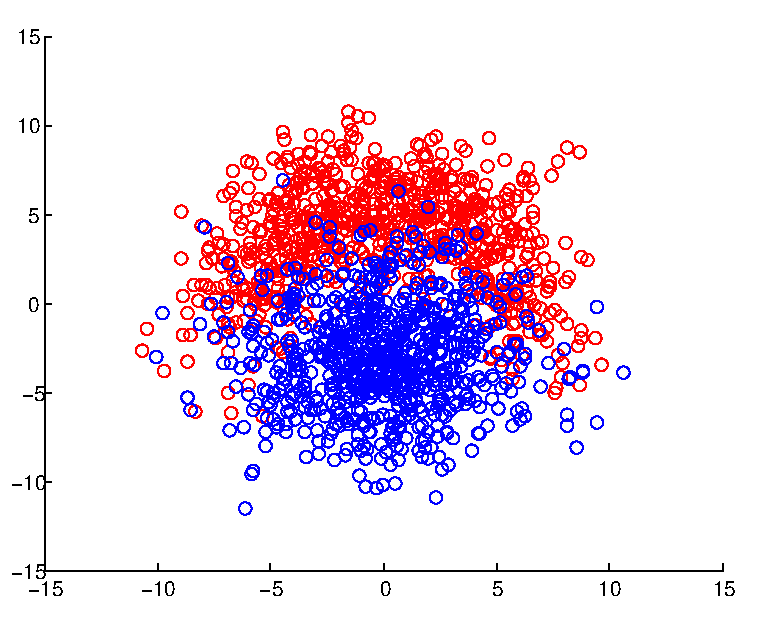
\includegraphics[width=0.75\textwidth]{images/data_scatterplot.pdf}
\caption{Data visualization.}
\label{data}
\end{figure}
In figure \ref{data} the data in the training set, which consists of the two classes, A (red) and B (blue).

\newpage
\section{k-Nearest Neighbours}
A kNN classifier, with $k = 1$, is trained on the trainings data. The performance is evaluated on the test data. This resulted in the following confusion matrix:
\begin{center}
\begin{tabular}{ | l | l | l | }
\hline
 & \textbf{True} & \textbf{False}\\
\hline
\textbf{Positive} & 206 & 44\\
\hline
\textbf{Negative} & 36 & 214\\
\hline
\end{tabular}
\end{center}
From the confusion matrix the error rate is computed by the following formula:
\begin{equation}
1 - accuracy = 1 - \frac{tp + fp}{tp + tn + fp + fn}
\end{equation}
The error rate and other statistical measures of the classifier are presented in the table below:
\begin{center}
\begin{tabular}{ | l | l | }
\hline
\textbf{Accuracy} & 84.0\%\\
\hline
\textbf{Precision} & 82.4\%\\
\hline
\textbf{Recall} & 85.1\%\\
\hline
\textbf{F-measure} & 83.7\%\\
\hline
\textbf{Error rate} & 16.0\%\\
\hline
\end{tabular}
\end{center}

\begin{figure}[!ht]
\centering
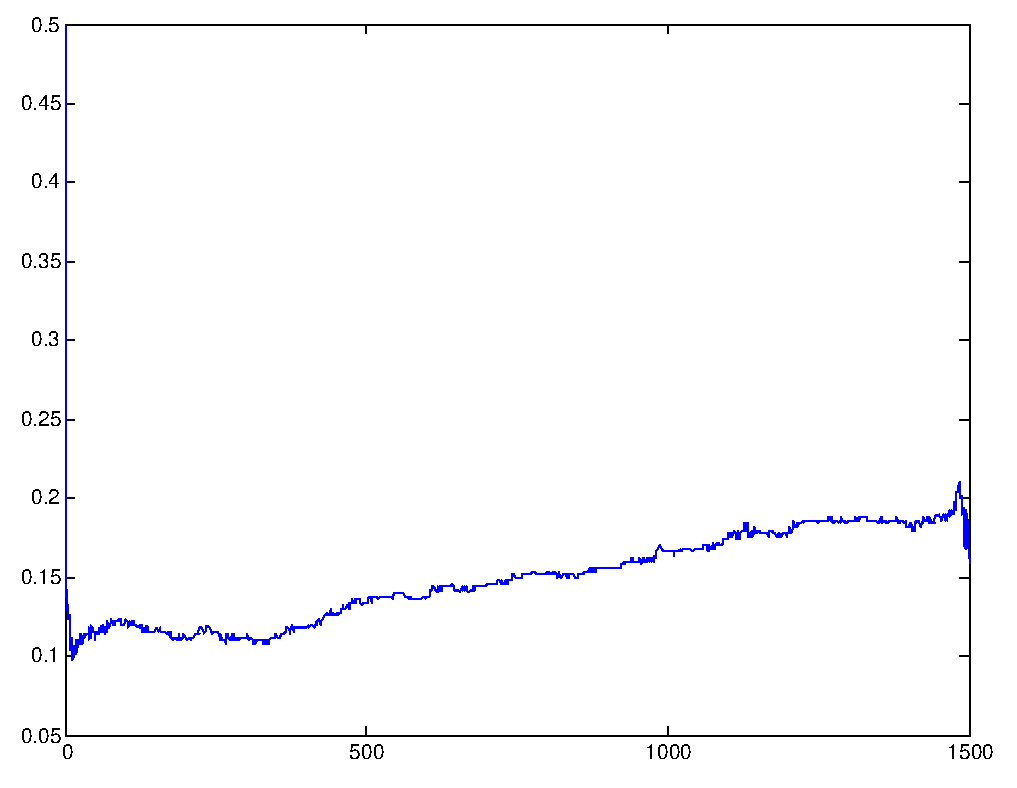
\includegraphics[width=0.75\textwidth]{images/error_rate_1500_1.pdf}
\caption{Graph of the error rate with various K}
\label{graph}
\end{figure}


\section{Cross Validation}


\end{document}